\chapter{React}\label{ch:react}

\section{Wat is React?}\label{sec:what}
	
	React is een JavaScript library gecreëerd door Facebook, React zou een oplossing bieden bij het ontwikkelen van complexe user interfaces met telkens veranderende datasets. Dit is geen onbelangrijke uitdaging en moet niet enkel onderhoudbaar zijn, maar ook schaalbaar zijn op het niveau van Facebook’s datasets.
	
	React werd geboren in de Facebook advertentie organisatie, waar men gebruik maakte van een traditionele client-side Model-View-Controller aanpak. Applicaties zoals deze maken normaal gezien gebruik ``van`` ``two-way data binding'' samen met renderen van het template. Telkens wanneer data objecten gewijzigd worden moet de pagina of een deel van de pagina opnieuw laden. In een kleine applicatie geeft dit geen merkbare problemen voor de performantie van de applicatie, maar hoe meer functionele uitbreidingen er aan de applicatie worden toegevoegd, hoe meer views en modellen de applicatie gaat bevatten. Deze zijn allemaal verbonden door een delicaat en onoverzichtelijk kluwen van code die de verbondenheid van views en modellen onderling bijhoudt. Dit wordt al snel enorm complex, moeilijk onderhoudbaar, moeilijk testbaar en niet-gebruiksvriendelijk omdat items die opgevraagd moeten worden vaak veel meer tijd vragen om gepresenteerd te kunnen worden.
	
	React werd dus ontwikkeld om één welbepaald probleem te gaan oplossen, nl. het tonen van data in de user interface. Als u denkt dat dat probleem reeds werd opgelost, bent u zeker niet verkeerd. Het verschil is dat React werd gecreëerd om grote schaalbare user interfaces, zoals Facebook en Instagram, met veel data die continu wijzigt te gaan behandelen. Dit soort interfaces kan gecreëerd worden en de data behandeling kan gebeuren via verschillende andere tools los van React, maar zorgen voor een hoop code en dus ook veel werk om te onderhouden en up-to-date te houden. Deze manier van werken werd reeds door Facebook zelf gebruikt want Facebook werd in 2004 al gemaakt, 9 jaar voor React werd uitgebracht. React zorgt met andere woorden eerder voor een korte, overzichtelijke en onderhoudbare manier van werken.
	
	React veranderde de manier waarop deze applicaties gecreëerd werden en voerde een aantal gewaagde veranderingen door op gebied van Web ontwikkeling. Toen React in mei 2013 op de markt werd gebracht was er heel wat commotie in de Web ontwikkeling community. Heel wat ontwikkelaars waren geïnteresseerd en sterk onder de indruk van de React aanpak maar sommigen waren niet tevreden met wat React deed. React daagde namelijk een aantal van de conventies uit, die reeds standaarden geworden zijn voor JavaScript frameworks.
	
	De ingenieurs bij Facebook hebben met React een mentaliteits wijziging doorgevoerd op gebied van web-ontwikkeling en het maken van schaalbare en onderhoudbare JavaScript applicaties. Ze voorzien React van een hele hoop nieuwe features die het bouwen van single-page applicaties toegankelijk maakt voor ontwikkelaars met verschillende kennis niveaus. \citep{gackenheimer:react}
	
\section{Recent framework}
	
	React wordt door velen vaak beschouwd als een volwaardig JavaScript framework vergelijkbaar met andere frameworks zoals Backbone, KnockoutJS, AngularJS, Ember, of één van de vele MVC frameworks die bestaan.
	
	\begin{figure}
		\centering
		\begin{tikzpicture}[every node/.style={draw,minimum width=25mm, minimum height=10mm,thick},>=latex]
			\node[top color=mvclightgreen, bottom color=mvcdarkgreen] (view)       at (0,0) {\color{white}View};
			\node[top color=mvclightorange,bottom color=mvcdarkorange](controller) at (3,3) {\color{white}Controller};
			\node[top color=mvclightred,   bottom color=mvcdarkred  ] (model)      at (6,0) {\color{white}Model};
			
			\draw[->,thick] (view.north) -- ($(controller.south west)!.25!(controller.south east)$);
			\draw[->,thick] (controller.south) -- ($(view.north west)!.75!(view.north east)$);
			\draw[->,thick] (controller.south) -- ($(model.north west)!.25!(model.north east)$);
			\draw[->,thick,dashed] ($(view.north east)!.7!(view.south east)$) -- ($(model.north west)!.7!(model.south west)$);
			\draw[->,thick] ($(model.north west)!.3!(model.south west)$) -- ($(view.north east)!.3!(view.south east)$);
		\end{tikzpicture}
		\caption{MVC basis architectuur}
		\label{fig:mvcbasis}
	\end{figure}
	
	\prettyref{fig:mvcbasis} toont de basis van een typische structuur van een MVC framework. Elk onderdeel heeft een eigen verantwoordelijkheid.
	
	\subsubsection*{Model-View-Controller:}
	\begin{itemize}
		\item \textbf{Model:} het model bevat de staat van een applicatie en stuurt events naar de View wanneer de staat van bepaalde data objecten werd gewijzigd.
		\item \textbf{View:} de view is de presentatie laag, dit is hetgeen de gebruiker ziet en bevat alle UI componenten. De view stuurt events naar controller en in sommige gevallen naar het model om bepaalde data op te halen.
		\item \textbf{Controller:} de controller zorgt ervoor dat alle events van de view en het model opgevangen worden, eventueel behandeld en op correcte wijze doorgestuurd worden naar de view of het model.
	\end{itemize}
	
	Dit is een slechts een oppervlakkige benadering van wat een MVC is, in realiteit zijn er verschillende varianten en implementaties, vandaar wordt er vaak verwezen naar een MV*- architectuur. Het is niet de bedoeling om uit te leggen wat MVC is, maar wat React juist niet is.
	
	Simpelweg beschouwd men React als de view in MV* - frameworks. Zoals eerder vermeld is React een manier om de user interface van een applicatie te beschrijven en een mechanisme om die user interface aan te passen wanneer de data wijzigt. React bestaat uit declaratieve componenten die samen een interface beschrijven en een data-binding mechanisme die niet observeerbaar is. React is ook heel makkelijk te manipuleren omdat je de gecreëerde componenten kan nemen en combineren met andere componenten, die telkens werken zoals je verwacht. Dit komt omdat React enorm schaalbaar is.
	
	In het artikel \cite{Harrington:React} worden drie JavaScript Frameworks vergeleken in verschillende browsers. \citeauthor{Harrington:React} schreef in elk framework een gelijkaardige applicatie (zie \prettyref{tbl:perfcompharrington}) die door een lijst van 1000 items loopt en elk item in de lijst weergeeft en in een listitem plaatst van een ``unsorted list'' in HTML. Wanneer op de run link (tekst label met milliseconden in) geklikt wordt, wordt de tijd opgeslagen en wanneer de 1000 elementen geladen zijn wordt opnieuw de tijd opgeslagen. De laatste tijd wordt van de eerste afgetrokken en de uitkomst wordt weergegeven op het scherm. Voor de test werd bij elk van de drie frameworks 10x de lijst geladen en werd de tijd bijgehouden in tabellen, dit werd voor drie browsers herhaald.
	
	\begin{table}
		\scriptsize
		\centering
		\begin{tabular}{@{}llll@{}}
			\toprule
				React \hfill \SI{40}{\milli\second} & Angular \hfill \SI{100}{\milli\second} & Knockout \hfill \SI{161}{\milli\second} & Raw \hfill \SI{14}{\milli\second} \\ \midrule
				pretty orange desk & odd brown house & short black bbq & fancy brown cookie \\
				helpful yellow house & fancy red keyboard & fancy white sandwich & fancy brown mouse \\
				big pink cookie & long black burger & long black car & handsome brown pony \\
				helpful orange burger & big pink mouse & tall white pizza & important brown pony \\
				clean orange house & important orange mouse & plain pink desk & odd brown mouse \\
				easy red cookie & handsome orange mouse & cheap brown house & mushy orange house \\
				tall red desk & plain orange sandwich & tall red bbq & small white burger \\
				crazy pink car & mushy blue sandwich & unsightly brown table & fancy yellow pizza \\
				crazy purple chair & expensive black bbq & long brown pony & inexpensive yellow bbq \\
				important orange sandwich & quaint orange chair & large pink chair & fancy purple chair \\
				mushy green table & clean blue pony & odd white chair & cheap brown desk \\
				plain yellow burger & odd yellow sandwich & mushy brown mouse & cheap black pizza \\
				small pink sandwich & large purple table & important yellow burger & pretty blue keyboard \\
				easy purple keyboard & important yellow pony & helpful white keyboard & handsome pink mouse \\
				inexpensive purple desk & unsightly red desk & clean black bbq & big orange cookie \\
				expensive red pizza & short brown table & small blue house & long pink house \\
				pretty yellow burger & expensive green bbq & angry green mouse & pretty yellow pizza \\
				adorable white cookie & quaint green mouse & small white cookie & quaint purple keyboard \\
			\bottomrule
		\end{tabular}
	\caption{Performance Comparison for React, Angular and Knockout, by Chris Harrington}
	\label{tbl:perfcompharrington}
	\end{table}
	
	\subsubsection*{Resultaten:}
	Het resultaat is dat over het gemiddelde React en Raw sneller laden dan Angular en Knockout. Dit resultaat is niet verassend, React en Raw JS hebben achterliggend niets meer te doen, terwijl Angular en Knockout eerst een aantal componenten eigen aan het framework moeten laten in haken zoals bv. Services, Directives,\ldots. React en Raw JS moeten dit niet doen waardoor ze sneller kunnen laden. Met deze test wil Harrington niet bewijzen dat React beter is dan Angular of Knockout maar wil hij de kracht van de schaalbaarheid van React aantonen.
	
	\begin{figure}
		\centering
		\subfloat{
			\scriptsize
			\begin{tabular}[b]{@{}rrrrr@{}} \toprule
				& React \hfill & Angular \hfill & Knockout \hfill & Raw \hfill \\
				\midrule
				& 58 & 236 & 282 & 8 \\
				& 563 & 254 & 367 & 42 \\
				& 34 & 324 & 362 & 40 \\
				& 35 & 271 & 316 & 41 \\
				& 24 & 228 & 340 & 42 \\
				& 23 & 312 & 340 & 41 \\
				& 26 & 261 & 335 & 38 \\
				& 25 & 219 & 327 & 42 \\
				& 22 & 293 & 335 & 39 \\
				& 24 & 254 & 344 & 40 \\
				\midrule
				Average & 83.4 & 265.2 & 334.8 & 37.3 \\
				\bottomrule
			\end{tabular}
		}
		\subfloat{
			\begin{tikzpicture}
				\begin{axis}[
					width  = 0.5*\textwidth,
					ybar=\pgflinewidth,
					xtick=\empty,
					bar width=2pt,
					ymajorgrids = true,
					ylabel = {Time (ms)},
					scaled y ticks = false,
					xmin=0.5,
					xmax=10.5,
					ytick={100,200,...,600},
					axis lines=left,
					enlargelimits=0,
					y tick style={draw=none},
					ymin=0,
					ymax=600,
					yticklabel pos=right
				]
					\addplot[style={bblue,fill=bblue,mark=none}] coordinates {(1,58) (2,563) (3,34) (4,35) (5,24) (6,23) (7,26) (8,25) (9,22) (10,24)};
					\addplot[style={bred,fill=bred,mark=none}] coordinates {(1,236) (2,254) (3,324) (4,271) (5,228) (6,312) (7,261) (8,219) (9,293) (10,254)};
					\addplot[style={byellow,fill=byellow,mark=none}] coordinates {(1,282) (2,367) (3,362) (4,316) (5,340) (6,340) (7,335) (8,327) (9,335) (10,344)};
					\addplot[style={bgreen,fill=bgreen,mark=none}] coordinates {(1,8) (2,42) (3,40) (4,41) (5,42) (6,41) (7,38) (8,42) (9,39) (10,40)};
				\end{axis}
			
				\begin{customlegend}[
					legend columns=-1,
					legend style={%
						draw=none,
						column sep=1ex},
					legend entries={%
						React,
						Angular,
						Knockout,
						Raw},
					legend style={%
						at={(6.4,-.2)},
						font=\scriptsize}
				]
					\addlegendimage{bblue,fill=bblue,area legend}
					\addlegendimage{bred,fill=bred,area legend}
					\addlegendimage{byellow,fill=byellow,area legend}
					\addlegendimage{bgreen,fill=bgreen,area legend,scale=.5}
				\end{customlegend}
			\end{tikzpicture}
		}
		\caption{Resultaat van performance test door  Chrome 39.0.2171.95}%
		\label{fig:reschrome}%
	\end{figure}
	
	\begin{figure}
		\centering
		\subfloat{
			\scriptsize
			\begin{tabular}[b]{@{}rrrrr@{}} \toprule
				& React \hfill & Angular \hfill & Knockout \hfill & Raw \hfill \\
				\midrule
				& 68 & 198 & 338 & 8 \\
				& 56 & 239 & 399 & 41 \\
				& 34 & 208 & 452 & 50 \\
				& 32 & 204 & 411 & 46 \\
				& 34 & 280 & 458 & 48 \\
				& 28 & 251 & 417 & 50 \\
				& 28 & 280 & 450 & 51 \\
				& 29 & 244 & 419 & 51 \\
				& 31 & 206 & 449 & 49 \\
				& 28 & 204 & 416 & 49 \\
				\midrule
				Average & 36.8 & 231.4 & 420.9 & 44.3 \\
				\bottomrule
			\end{tabular}
		}
		\subfloat{
			\begin{tikzpicture}
				\begin{axis}[
					width  = 0.5*\textwidth,
					ybar=\pgflinewidth,
					xtick=\empty,
					bar width=2pt,
					ymajorgrids = true,
					ylabel = {Time (ms)},
					scaled y ticks = false,
					xmin=0.5,
					xmax=10.5,
					ytick={100,200,...,600},
					axis lines=left,
					enlargelimits=0,
					y tick style={draw=none},
					ymin=0,
					ymax=600,
					yticklabel pos=right
				]
					\addplot[style={bblue,fill=bblue,mark=none}] coordinates {(1,68) (2,56) (3,34) (4,32) (5,34) (6,28) (7,28) (8,29) (9,31) (10,28)};
					\addplot[style={bred,fill=bred,mark=none}] coordinates {(1,198) (2,239) (3,208) (4,204) (5,280) (6,251) (7,280) (8,244) (9,206) (10,204)};
					\addplot[style={byellow,fill=byellow,mark=none}] coordinates {(1,338) (2,399) (3,452) (4,411) (5,458) (6,417) (7,450) (8,419) (9,449) (10,416)};
					\addplot[style={bgreen,fill=bgreen,mark=none}] coordinates {(1,8) (2,41) (3,50) (4,46) (5,48) (6,50) (7,51) (8,51) (9,49) (10,49)};
				\end{axis}
			
				\begin{customlegend}[
					legend columns=-1,
					legend style={%
						draw=none,
						column sep=1ex},
					legend entries={%
						React,
						Angular,
						Knockout,
						Raw},
					legend style={%
						at={(6.4,-.2)},
						font=\scriptsize}
				]
					\addlegendimage{bblue,fill=bblue,area legend}
					\addlegendimage{bred,fill=bred,area legend}
					\addlegendimage{byellow,fill=byellow,area legend}
					\addlegendimage{bgreen,fill=bgreen,area legend,scale=.5}
				\end{customlegend}
			\end{tikzpicture}
		}
		\caption{Resultaat van performance test door Chris Harrington voor Firefox 34.0.5}%
		\label{fig:resfirefox}%
	\end{figure}
	
	\begin{figure}
		\centering
		\subfloat{
			\scriptsize
			\begin{tabular}[b]{@{}rrrrr@{}} \toprule
				& React \hfill & Angular \hfill & Knockout \hfill & Raw \hfill \\
				\midrule
				& 51 & 82 & 138 & 16 \\
				& 37 & 121 & 193 & 65 \\
				& 28 & 114 & 187 & 65 \\
				& 26 & 120 & 171 & 65 \\
				& 26 & 117 & 182 & 66 \\
				& 30 & 118 & 175 & 62 \\
				& 25 & 120 & 173 & 64 \\
				& 28 & 114 & 173 & 66 \\
				& 26 & 113 & 173 & 63 \\
				& 26 & 117 & 178 & 64 \\
				\midrule
				Average & 30.3 & 113.6 & 174.3 & 59.6 \\
				\bottomrule
			\end{tabular}
		}
		\subfloat{
			\begin{tikzpicture}
				\begin{axis}[
					width  = 0.5*\textwidth,
					ybar=\pgflinewidth,
					xtick=\empty,
					bar width=2pt,
					ymajorgrids = true,
					ylabel = {Time (ms)},
					scaled y ticks = false,
					xmin=0.5,
					xmax=10.5,
					ytick={100,200,...,600},
					axis lines=left,
					enlargelimits=0,
					y tick style={draw=none},
					ymin=0,
					ymax=600,
					yticklabel pos=right
				]
					\addplot[style={bblue,fill=bblue,mark=none}] coordinates {(1,51) (2,37) (3,28) (4,26) (5,26) (6,30) (7,25) (8,28) (9,26) (10,26)};
					\addplot[style={bred,fill=bred,mark=none}] coordinates {(1,82) (2,121) (3,114) (4,120) (5,117) (6,118) (7,120) (8,114) (9,113) (10,117)};
					\addplot[style={byellow,fill=byellow,mark=none}] coordinates {(1,138) (2,193) (3,187) (4,171) (5,182) (6,175) (7,173) (8,173) (9,173) (10,178)};
					\addplot[style={bgreen,fill=bgreen,mark=none}] coordinates {(1,16) (2,65) (3,65) (4,65) (5,66) (6,62) (7,64) (8,66) (9,63) (10,64)};
				\end{axis}
			
				\begin{customlegend}[
					legend columns=-1,
					legend style={%
						draw=none,
						column sep=1ex},
					legend entries={%
						React,
						Angular,
						Knockout,
						Raw},
					legend style={%
						at={(6.4,-.2)},
						font=\scriptsize}
				]
					\addlegendimage{bblue,fill=bblue,area legend}
					\addlegendimage{bred,fill=bred,area legend}
					\addlegendimage{byellow,fill=byellow,area legend}
					\addlegendimage{bgreen,fill=bgreen,area legend,scale=.5}
				\end{customlegend}
			\end{tikzpicture}
		}
		\caption{Resultaat van performance test door Chris Harrington voor Safari 7.0.2}%
		\label{fig:ressafari}%
	\end{figure}
	
\section{React concepten}
		
	De React API is klein en daardoor gemakkelijk aan te leren. Gemakkelijk wil niet zeggen dat het herkenbaar is. Eerst moeten er een aantal concepten en terminologie worden uitgelegd.

\section{Componenten}
	
	Componenten zijn de basis van React en de view van de applicatie. Hieronder vindt je een simpel voorbeeld van zo’n component. Let goed op bij de `render' functie, deze geeft een HTML tag terug. Wanneer deze zal aangeroepen worden zal die de tekst ``Hello world'' laten verschijnen op de HTML pagina.
	
	\reactcode{code/componenten.js}{TODO: add caption}{code:comp}

\section{Virtual DOM}
	
	Dit is waarschijnlijk het meest belangrijke concept van React. Het virtuele DOM is de oplossing voor het probleem die het DOM stelt, namelijk dat het (nog) niet aangepast werd voor het weergeven van dynamische data. Met JavaScript en JQuery kon je als ontwikkelaar wel een oplossing voor dit probleem vinden, maar dat bleek zowieso een hele hoop werk en er kwam heel wat code en denkwerk bij kijken. Dit was uiteraard het probleem waarvoor Facebook React heeft ontwikkeld. Het virtuele DOM is geen nieuw concept en bestaat al eerder dan React, React is wel ontwikkeld met het concept van het virtuele DOM in het achterhoofd.
	
	Het virtuele DOM wordt ontwikkeld bovenop het DOM, het gaat uiteraard het DOM gaan behandelen maar doet dit zo weinig en zo efficiënt mogelijk, door te werken met een light weight kopie van het DOM. Wanneer de data wordt gewijzigd in de kopie wordt er gekeken welke delen in het DOM vervangen moeten worden. Er wordt opzoek gegaan naar de kortste manier om de gewijzigde delen te gaan vervangen. Deze manier gaat veel sneller dan direct te werken met het DOM, omdat niet alle delen van het DOM die belastend zijn voor de browser her-in-ge-laden moeten worden.\citep{gackenheimer:react}
	
	Om dit te realiseren maakt React gebruik van diff algoritmes, event delegation en rendering.
	
	\subsection{Diff algoritmen}
		
		React gaat via een aantal algoritmen op zoek naar het minimum aantal stappen die nodig zijn om van de vorige versie van het DOM naar een nieuwere versie te gaan.
		\begin{itemize}
			\item Level per level: React gaat proberen om op level niveau wijzigingen aan te brengen, dit gaat de complexiteit drastisch verminderen en brengt weinig verlies met zich mee omdat het zeer zeldzaam is in web applicaties dat componenten verplaatst worden naar een ander niveau in de boom structuur. Zie \prettyref{fig:levelperlevel}.
			\begin{figure}
				\centering
				\begin{tikzpicture}[decoration={random steps,segment length=1mm,amplitude=0.5pt},ultra thick,every node/.style={draw,circle,decorate,inner sep=5}]
					\ECFJD
					\node (A) at (0,0) {};
					\node (B) at (1,0) {};
					\node (C) at (.5,1) {};
					\node (D) at (1.5,2) {};
					\node (E) at (2.5,1) {};
					\node (F) at (2,0) {};
					\node (G) at (3,0) {};
					
					\node (H) at (5,0) {};
					\node (I) at (6,0) {};
					\node (J) at (5.5,1) {};
					\node (K) at (6.5,2) {};
					\node (L) at (7.5,1) {};
					\node (M) at (7,0) {};
					\node (N) at (8,0) {};
					
					\draw[decorate] (A) -- (C) (B) -- (C) (C) -- (D) (D) -- (E) (F) -- (E) (E) -- (G);
					\draw[decorate] (H) -- (J) (I) -- (J) (J) -- (K) (K) -- (L) (M) -- (L) (L) -- (N);
					
					\draw[tikzorange,decorate] (-.4,-.4) -- (-.4,.4) -- (1.4,.4) -- (1.4,-.4) -- cycle;
					\draw[tikzorange,decorate] (4.6,-.4) -- (4.6,.4) -- (6.4,.4) -- (6.4,-.4) -- cycle;
					\draw[tikzorange,decorate] (.5,-.4) -- (.5,-.8) -- (5.5,-.8) -- (5.5,-.4);
						
					\draw[tikzlightblue,decorate] (1.6,-.4) -- (1.6,.4) -- (3.4,.4) -- (3.4,-.4) -- cycle;
					\draw[tikzlightblue,decorate] (6.6,-.4) -- (6.6,.4) -- (8.4,.4) -- (8.4,-.4) -- cycle;
					\draw[tikzlightblue,decorate] (2.5,-.4) -- (2.5,-1.2) -- (7.5,-1.2) -- (7.5,-.4);
					
					\draw[tikzpurple,decorate] (.1,.6) -- (.1,1.4) -- (2.9,1.4) -- (2.9,.6) -- cycle;
					\draw[tikzpurple,decorate] (5.1,.6) -- (5.1,1.4) -- (7.9,1.4) -- (7.9,.6) -- cycle;
					\draw[tikzpurple,decorate] (2.9,1) -- (5.1,1);
					
					\draw[tikzdarkblue,decorate] (.7,1.6) -- (.7,2.4) -- (2.3,2.4) -- (2.3,1.6) -- cycle;
					\draw[tikzdarkblue,decorate] (5.7,1.6) -- (5.7,2.4) -- (7.3,2.4) -- (7.3,1.6) -- cycle;
					\draw[tikzdarkblue,decorate] (2.3,2) -- (5.7,2);
					
					\node[draw=none,rectangle] at (1.5,2.75) {Voor};
					\node[draw=none,rectangle] at (6.5,2.75) {Na};
				\end{tikzpicture}
				\caption{Level per level aanpassen}%
				\label{fig:levelperlevel}%
			\end{figure}
			\item Lijsten: Wanneer een component bij een éénmalige iteratie 5 andere componenten bevat wordt het moeilijk om in het midden van die lijst een nieuwe component toe te voegen. React gaat standaard een associatie maken tussen het eerste component van de eerste lijst en het eerste component van de tweede lijst, etc. Als ontwikkelaar kan je React helpen door een sleutel attribuut toe te voegen zodat React een beter begrip krijgt over de mapping van beide lijsten.
			\begin{figure}
				\centering
				\begin{tikzpicture}[decoration={random steps,segment length=1mm,amplitude=0.5pt},ultra thick,every node/.style={draw,circle,decorate,inner sep=5}]
					\ECFJD
					\node (A) at (0.00,0) {};
					\node (B) at (0.75,0) {};
					\node (C) at (1.50,0) {};
					\node (D) at (2.25,0) {};
					\node (E) at (3.00,0) {};
					\node[tikzdarkblue] (F) at (3.75,0) {};
					\node (G) at (0.25,1.5) {};
					\node (H) at (1.00,1.5) {};
					\node (I) at (1.75,1.5) {};
					\node (J) at (2.50,1.5) {};
					\node (K) at (3.25,1.5) {};
					
					\draw[decorate] (A) -- (G) (B) -- (H) (C) -- (I) (D) -- (J) (E) -- (K);
					\node[draw=none,rectangle] at (1.75,2.25) {Zonder keys};
					
					\node[inner sep=3] (L) at (5.25,0) {a};
					\node[inner sep=3] (M) at (6.00,0) {b};
					\node[inner sep=3] (N) at (6.75,0) {c};
					\node[tikzdarkblue,inner sep=3] (O) at (7.50,0) {z};
					\node[inner sep=3] (P) at (8.25,0) {d};
					\node[inner sep=3] (Q) at (9.00,0) {e};
					\node[inner sep=3] (R) at (5.50,1.5) {a};
					\node[inner sep=3] (S) at (6.25,1.5) {b};
					\node[inner sep=3] (T) at (7.00,1.5) {c};
					\node[inner sep=3] (U) at (7.75,1.5) {d};
					\node[inner sep=3] (V) at (8.50,1.5) {e};
					
					\draw[decorate] (L) -- (R) (M) -- (S) (N) -- (T) (P) -- (U) (Q) -- (V);
					\node[draw=none,rectangle] at (7.00,2.25) {Met keys};
				\end{tikzpicture}
				\caption{Lijsten}%
				\label{fig:lijsten}%
			\end{figure}
		\end{itemize}
	
	\subsection{Event delegation}
		
		Toevoegen van event listeners aan DOM nodes is enorm traag en gaat veel geheugen gebruiken. React gebruikt hiervoor een populaire techniek genaamd ``event delegation''. Bij event delegation wordt een event getriggerd op de parent node en niet op elke child node bv. Onclick listener op een unsorted list ($<$ul$>$) element in plaats van op elk list item ($<$li$>$) element in de list . Wanneer het event wordt getriggerd gaat de parent nagaan welk child element wordt aangeklikt en op basis van het id, die React automatisch toevoegd aan elk child element, de nodige wijzigingen doorvoeren.
	
	\subsection{Rendering}
		
		Wanneer setState wordt aangeroepen op een component, zal React dat component aanduiden als ``Dirty''. Aan het einde van elke event loop zal React alle ``dirty'' componenten opnieuw laden. Dit betekent dat er tijdens een event loop, er slechts 1 moment is dat het DOM wordt ge-update. Dit is een belangrijke eigenschap om performante applicaties te schrijven, maar is extreem moeilijk te benaderen in gewone JavaScript code, React regelt dit standaard voor de ontwikkelaar.
		
		Het voordeel is dat setState niet alleen op het root element kan opgeroepen worden, maar op elk child element aanwezig in de applicatie. Wanneer hierop een wijziging gebeurt moet niet het volledige DOM worden overschreven maar slechts een deel van de tree.
		
		\begin{figure}
			\centering
			\resizebox{.99\linewidth}{!}{
			\begin{tikzpicture}[decoration={random steps,segment length=1mm,amplitude=0.5pt},ultra thick,every node/.style={draw,circle,decorate,inner sep=4}]
				\ECFJD
				\node (sA) at (0.00,0) {};
				\node (sB) at (0.50,1) {};
				\node (sC) at (1.00,0) {};
				\node (sD) at (1.50,2) {};
				\node (sE) at (2.00,1) {};
				\node (sF) at (2.50,3) {};
				\node (sG) at (2.50,0) {};
				\node (sH) at (3.00,1) {};
				\node (sI) at (3.50,2) {};
				\node (sJ) at (3.50,0) {};
				\node (sK) at (4.00,1) {};
				
				\draw[decorate] (sA) -- (sB) (sB) -- (sC) (sB) -- (sD) (sD) -- (sE) (sD) -- (sF) (sF) -- (sI) (sI) -- (sH) (sI) -- (sK) (sH) -- (sG) (sH) -- (sJ);
				\node[draw=none,rectangle] at (2.50,3.75) {setState};
				
				\draw[->,red,decorate] ($(sB.north)+(0,1)$) -- (sB.north);
				\draw[->,red,decorate] ($(sA.west)-(1,0)$) -- (sA.west);
				\draw[->,red,decorate] ($(sB.north west)+(-.7071,.7071)$) -- (sB.north west);
				\draw[->,red,decorate] ($(sA.north west)+(-.7071,.7071)$) -- (sA.north west);
				\draw[->,red,decorate] ($(sB.south east)+(.866,-.5)$) -- (sB.south east);
				\draw[->,red,decorate] ($(sI.north east)+(.7071,.7071)$) -- (sI.north east);
				
				\node[fill=red] (dA) at (5.00,0) {};
				\node[fill=red] (dB) at (5.50,1) {};
				\node (dC) at (6.00,0) {};
				\node (dD) at (6.50,2) {};
				\node (dE) at (7.00,1) {};
				\node (dF) at (7.50,3) {};
				\node (dG) at (7.50,0) {};
				\node (dH) at (8.00,1) {};
				\node[fill=red] (dI) at (8.50,2) {};
				\node (dJ) at (8.50,0) {};
				\node (dK) at (9.00,1) {};
				
				\draw[decorate] (dA) -- (dB) (dB) -- (dC) (dB) -- (dD) (dD) -- (dE) (dD) -- (dF) (dF) -- (dI) (dI) -- (dH) (dI) -- (dK) (dH) -- (dG) (dH) -- (dJ);
				\node[draw=none,rectangle] at (7.50,3.75) {Dirty};
				
				\node[fill=blue] (rA) at (10.00,0) {};
				\node[fill=blue] (rB) at (10.50,1) {};
				\node[fill=blue] (rC) at (11.00,0) {};
				\node (rD) at (11.50,2) {};
				\node (rE) at (12.00,1) {};
				\node (rF) at (12.50,3) {};
				\node[fill=blue] (rG) at (12.50,0) {};
				\node[fill=blue] (rH) at (13.00,1) {};
				\node[fill=blue] (rI) at (13.50,2) {};
				\node[fill=blue] (rJ) at (13.50,0) {};
				\node[fill=blue] (rK) at (14.00,1) {};
				
				\draw[decorate] (rA) -- (rB) (rB) -- (rC) (rB) -- (rD) (rD) -- (rE) (rD) -- (rF) (rF) -- (rI) (rI) -- (rH) (rI) -- (rK) (rH) -- (rG) (rH) -- (rJ);
				\node[draw=none,rectangle] at (12.50,3.75) {Re-rendered};
			\end{tikzpicture}
			}
			\caption{Flow setState to render DOM}%
			\label{fig:setstateflow}%
		\end{figure}
		
		Deze technieken zijn niet nieuw en worden gebruikt door andere JavaScript libraries en frameworks:
		
		\begin{itemize}
			\item \textbf{Virtual-dom by Matt Esch:} Een JavaScript virtual dom algoritme
			\item \textbf{Mithril:} JavaScript Framework
			\item \textbf{Bobril:} component georiënteerd framework geïnspireerd door React en Mithril.
		\end{itemize}
		
		Wat React speciaal maakt hierin is dat wanneer je als ontwikkelaar de logische volgorde volgt die nodig is om een applicatie te bouwen in React, je dit allemaal standaard krijgt en zelf hiervoor niets hoeft te doen.
	
	\subsection{JSX}
		
		JSX is de transformatie laag van React om XML syntax die gebruikt wordt om React componenten te schrijven om te zetten naar syntax die door React gebruikt wordt om elementen te renderen in JavaScript. Let op! Dit is geen verplicht onderdeel van React maar wordt sterk aangeraden om het te gebruiken. JSX maakt coderen veel eenvoudiger en leesbaarder, zo kan je bijvoorbeeld HTML tags meegeven en aanvaard het aangepaste React klassen.
		
		\reactcode{code/jsx.js}{TODO: add caption}{code:jsx}
	
	\subsection{Properties}
		
		Properties zijn een set van opties die een component bevat en worden aangeroepen in React als ``this.props'', een gewoon JavaScript object in React. Properties zullen tijdens de lifecycle van een component niet wijzigen, ze zijn immutable. Wanneer een ontwikkelaar iets wil wijzigen aan een component zal hij de state van een object moeten wijzigen.
	
	\subsection{State}
		
		State is een set op elke component die geïnitialiseerd kan worden op elke component en die gewijzigd kan worden doorheen de lifecycle van van dat component. De state mag niet gewijzigd worden buiten het component tenzij door een parent component. Het is aangewezen om zo weinig mogelijk state objecten te gebruiken op de componenten, hoe meer state objecten geïnitialiseerd en aangepast worden hoe groter de complexiteit van de componenten wordt.
	
	\subsection{Flux}
		
		Flux is een project dat zeer nauw verbonden is met React. Het is belangrijk om te weten hoe het werkt met React. Flux is de Facebook applicatie architectuur voor hoe data werkt met React componenten op een logische en georganiseerde manier. Flux is geen MVC architectuur omdat het niet werkt met bi-directionele data flow. Flux is daarentegen wel essentieel voor React omdat het helpt met het gebruik van React componenten op de manier waarop ze voorzien zijn om gebruikt te worden. Flux doet dit door een uni-directionele data flow te gaan creëren die door drie stukken van de flux architectuur wordt geleid nl. de dispatcher, de stores en uiteindelijk de React View. Flux is essentieel in het bouwen van webapplicaties met React en zal dus niet verder aan bod komen in deze scriptie.

\section{React Core}
	
	Tot hiertoe werd een beeld gecreëerd over hoe React werkt en zich profileert ten opzichte van andere frameworks. Er werden een aantal concepten verklaard die hieronder in detail worden uitgediept. In dit hoofdstuk wordt de syntax van React belangrijk en worden enkele basis begrippen in detail uitgelegd aan de hand van React code, vooral in de JSX syntax.
	
	\subsection{React.createClass}
		
		In het hoofdstuk over React Concepten werd aangehaald dat componenten de basis vormen van een React applicatie. De methode \emph{React.createClass} zorgt ervoor dat een nieuwe component wordt aangemaakt, deze methode moet verplicht de methode \emph{render()} overschrijven omdat deze het object, meestal in HTML vorm weergeeft. De \emph{render()} methode zal later verder toegelicht worden.
		
		\reactcode{code/mycomponent.js}{TODO: add caption}{code:mycomponent}
		
		In \prettyref{code:mycomponent} wordt een basis object `MyComponent' aangemaakt via de methode \emph{React.createClass} door de \emph{render()} methode te overschrijven zal een <div> element aangemaakt worden die de tekst ``Hello world'' op het scherm afprint. Op lijn 8 wordt \emph{React.render()} methode opgeroepen die het object zal creëren en aan het DOM zal toevoegen als child node van de node met id ``container''.
		
		Wanneer een waarde aan het component moet worden doorgegeven gaan we volgende syntax krijgen:
		
		\reactcode{code/propertyname.js}{TODO: add caption}{code:propertyname}
		
		Wanneer in de methode \emph{React.render} het object \emph{myComponent} wordt aangemaakt geven we een property `name' mee. In \emph{myComponent} wordt verwezen naar de property name door gebruik te maken van ``\{this.props.name\}'' om een property op te roepen.
	
	\subsection{React.Children}
		
		\emph{React.Children} is een object die een aantal helper functies bevat om gemakkelijker te werken met de properties van een component (\emph{this.props.children}). Deze functies zullen uitgevoerd op elk child object die de component bevat en geven een object terug.
		
		\begin{itemize}
			\item \emph{React.Children.map( children, myFn, [, context] )}: Deze functie zal voor elk child object in \emph{children} de functie \emph{myFn} uitvoeren, waarbij (optioneel) een context kan toegevoegd worden.
			\reactcode{code/mapfunctie.js}{TODO: add caption}{code:mapfunctie}
			\prettyref{code:mapfunctie} toont aan hoe de map functie werkt door twee child elementen toe te voegen wanneer een object van \emph{MyComponent} wordt geïnitialiseerd. In de \emph{render} functie van \emph{MyComponent} wordt elk child object van \emph{this.props.children} overlopen en voor elk child object wordt de info in de console uitgeprint (zie \prettyref{fig:mapconsole}).
			\begin{figure}%
				\centering
				\fbox{
					\resizebox{.9\linewidth}{!}{
						\begin{tikzpicture}
							\node[anchor=west] at (0,.6) {\texttt{Object \{{\color{consolepurple}\$\$typeof}: {\color{consoleorange}Symbol(react.element)}, {\color{consolepurple}type}: {\color{consoleorange}\textquotedbl p\textquotedbl}, {\color{consolepurple}key}: {\color{consoleorange}\textquotedbl first\textquotedbl}, {\color{consolepurple}ref}: null, {\color{consolepurple}props}: Object...\}}};
							\node at (24,.6) {\texttt{script.js:62}};
							\node[anchor=west] at (0,0) {\texttt{Object \{{\color{consolepurple}\$\$typeof}: {\color{consoleorange}Symbol(react.element)}, {\color{consolepurple}type}: {\color{consoleorange}\textquotedbl p\textquotedbl}, {\color{consolepurple}key}: {\color{consoleorange}\textquotedbl second\textquotedbl}, {\color{consolepurple}ref}: null, {\color{consolepurple}props}: Object...\}}};
							\node at (24,0) {\texttt{script.js:62}};
						\end{tikzpicture}
					}
				}
				\caption{Console.log function on child}%
				\label{fig:mapconsole}%
			\end{figure}
			\item \emph{React.Children.forEach( children, myFn [, context])}: \emph{forEach} functie werkt net zoals \emph{map} functie maar geeft geen object terug. Deze functie zal enkel de lijst doorlopen en een actie uitvoeren op elk child object.
			\item \emph{React.Children.count( children )}: de \emph{count} methode zal het aantal child objecten in de lijst children terug geven.
		\end{itemize}
	
	\subsection{React.createElement}
		
		De \emph{createElement} methode wordt gebruikt om een \emph{ReactElement} te creëren, deze elementen verhogen de performantie van een React applicatie, omdat ze kunnen kunnen bestaan uit ReactElementen, ReactComponenten, HTML tags, \ldots.
		
		\begin{itemize}
			\item[] \emph{React.createElement( type, [ props [, children … ]] )}
		\end{itemize}
		
		Een element wordt gecreëerd met minstens één, en optioneel drie argumenten. Een string type, optioneel een lijst van properties en optioneel een lijst van child objecten.
		
		\reactcode{code/createelement.js}{TODO: add caption}{code:createelement}
		
		In \prettyref{code:createelement} wordt op lijn 4 een <div> element expliciet gecreëerd terwijl eenzelfde functie op lijn 11 wordt aangeroepen met als type een object van \emph{MyComponent}. In dit voorbeeld lijkt het overbodig om de functie op te roepen om een <div> element aan te maken maar wanneer de elementen gaan nesten en de complexiteit van de user interface begint te stijgen is het aangeraden om met \emph{ReactElementen} te gaan werken.
	
\section{React componenten}
	
	React componenten zijn de bouwstenen van een React applicatie. React componenten hebben een eigen API die een aantal methodes en helpers bevat.
	
	\subsection{Creatie}
		
		Een React component kan op verschillende manieren aangemaakt worden, hieronder vindt u twee voorbeelden van de meest gebruikte manieren.
		
		\begin{itemize}
			\item Voorbeeld 1: \emph{React.Component} als super klasse, maak een klasse aan die overerft van \emph{React.Component}. Overschrijf \textbf{altijd} de \emph{render()} methode (zie \prettyref{code:vb1}).
			\reactcode{code/vb1.js}{TODO: add caption}{code:vb1}
			\item Voorbeeld 2: maak een variabele die de methode \emph{React.createClass} aanroept, deze methode geeft een object weer van type \emph{React.Component} met eigen implementatie (zie \prettyref{code:vb2}). Deze manier is de meest gebruikte manier om een component aan te maken.
			\reactcode{code/vb2.js}{TODO: add caption}{code:vb2}
		\end{itemize}
	
	\subsection{State}
		
		De State van een property kan gewijzigd worden door de functie \emph{setState} aan te roepen in een component. Deze functie kan een andere functie aanroepen of een object weergegeven die de state van de component wijzigt. Wanneer \emph{setState} aangeroepen wordt, komt het nieuwe object in de React update queue, het mechanisme die React gebruikt om wijzigingen te behandelen. (Zie Virtual DOM, Rendering)
		
		Door deze manier van werken moet men als ontwikkelaar rekening houden met een aantal zaken wanneer \emph{setState} wordt aangeroepen. Zo is er geen enkele garantie dat de updates in een bepaalde volgorde zullen gebeuren. Wanneer er een afhankelijkheid is voor het updaten van een bepaalde property kan dit via een Callback functie worden doorgegeven die optioneel wordt meegegeven aan \emph{setState}. Daarnaast is het aangewezen om de state niet te wijzigen met de ``dot-notatie'' \emph{this.state}, en deze enkel te gebruiken om de state op te roepen. Het idee hierachter is dat de ontwikkelaar het state object als immutable moet beschouwen en enkel het \emph{setState} proces van React de wijzigingen aan de state controleert.
	
	\subsection{Specificatie functies en component LifeCycle}
		
		Specificatie functies zijn functies die verplicht of optioneel kunnen worden toegevoegd aan componenten wanneer ze worden geinitialiseerd, sommigen ervan zijn lifecycle functies. Er zijn drie soorten lifecycles mogelijk op een component:
		
		\begin{itemize}
			\item De eerste keer wanneer een component aan het DOM wordt toegevoegd.
			\item Wanneer de state wijzigt.
			\item Wanneer de properties wijzigen.
		\end{itemize}
		
		\begin{figure}
			\centering
			\begin{tikzpicture}[every node/.style={anchor=south west},>=latex]
				\node[draw,minimum width=5cm,minimum height=6.75cm] at (0,0) {};
				\node[draw=floworange,fill=floworange,minimum width=5cm,minimum height=1cm] at (0,6.75) {\color{white}First Render};
				\node[draw=flowblue,fill=flowblue,rounded corners,minimum width=4cm, minimum height=.75cm] (A) at (.5,.5) {\color{white}componentDidMount};
				\node[draw=flowblue,fill=flowblue,rounded corners,minimum width=4cm, minimum height=.75cm] (B) at (.5,1.75) {\color{white}render};
				\node[draw=flowblue,fill=flowblue,rounded corners,minimum width=4cm, minimum height=.75cm] (C) at (.5,3) {\color{white}componentWillMount};
				\node[draw=flowblue,fill=flowblue,rounded corners,minimum width=4cm, minimum height=.75cm] (D) at (.5,4.25) {\color{white}getInitialState};
				\node[draw=flowblue,fill=flowblue,rounded corners,minimum width=4cm, minimum height=.75cm] (E) at (.5,5.5) {\color{white}getDefaultProps};
				\draw[->,thick,floworange] (B) -- (A);
				\draw[->,thick,floworange] (C) -- (B);
				\draw[->,thick,floworange] (D) -- (C);
				\draw[->,thick,floworange] (E) -- (D);
			\end{tikzpicture}
			\caption{Lifecycle first render}%
			\label{fig:lifecyclefirstrender}%
		\end{figure}
	
	\subsection{Render}
		
		Zoals reeds een aantal keren vermeld moet elke component een render functie bevatten. Deze functie aanvaardt een \emph{ReactElement} en voorziet een container locatie waar het component zal toegevoegd worden aan het DOM.
	
	\subsection{getInitialState}
		
		Deze functie zal een object teruggeven, de inhoud van dit object zal de state van het component setten wanneer het voor de eerste keer geinitialiseerd wordt.
		
		\reactcode{code/getinitialstate.js}{TODO: add caption}{code:getinitialstate}
		
		\prettyref{code:getinitialstate} geeft een object \emph{MyComponent} weer waarbij een <div> element met de tekst ``Hello Steven'' wordt toegevoegd aan het DOM. Door \emph{getInitialState} aan te roepen, kan de name property een start waarde mee krijgen.
	
	\subsection{getDefaultProps}
		
		Wanneer een \emph{ReactClass} (component of element) voor het eerst wordt aangemaakt, wordt de methode \emph{getDefaultProps} éémalig aangeroepen om de properties op de component met default waarden te bevolken. Wanneer deze methode niet opgeroepen wordt zullen \emph{this.props} voorzien worden van \emph{null} waarden of de waarde die tijdens de initialisatie worden meegegeven. (<MyComponent name = \textquotedbl Steven\textquotedbl />).
	
	\subsection{componentWillMount}
		
		\emph{ComponentWillMount} is een lifeCycle event die React gebruikt wanneer React het component neemt en op het DOM plaatst. De methode wordt éénmaal aangeroepen vlak voor de \emph{render} methode van de component. Het unieke aan componentWillMount is dat wanneer de ontwikkelaar \emph{setState} aanroept in de methode en de \emph{state} van het component wijzigt er niet opnieuw wordt ingeladen, maar dat de gewijzigde state onmiddellijk zichtbaar is.
	
	\subsection{componentDidMount}
		
		ComponentDidMount is een methode die enkel aan de client kant wordt aangeroepen. De component bestaat en staat in het DOM.
	
	\subsection{Mixin}
		
		Een Mixin is een array, het kan de lifecycle events van een component monitoren zodat de ontwikkelaar met zekerheid weet dat functionaliteit op de correcte manier en tijdstippen van de lifecycle kan uitgevoerd worden. \prettyref{code:mixin} toont hoe een Mixin een component kan monitoren. Deze code zal een timer genereren die de levensduur van de component op pagina weergeeft in het aantal seconden (zie \prettyref{fig:timer}).
		
		\reactcode{code/mixin.js}{TODO: add caption}{code:mixin}
		
		\begin{figure}
			\centering
			\fbox{
				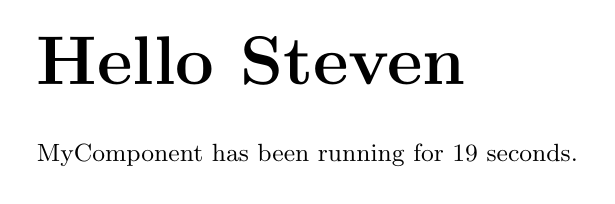
\begin{tikzpicture}
					\node[anchor=west] at (0,1.2) {\rmfamily\Huge\bfseries Hello Steven};
					\node[anchor=west] at (0,0) {\rmfamily\small MyComponent has been running for 19 seconds.};
				\end{tikzpicture}
			}
			\caption{Screenshot resultaat mixin voorbeeld}%
			\label{fig:timer}%
		\end{figure}
		
		\begin{figure}
			\centering
			\begin{tikzpicture}[every node/.style={anchor=south west},>=latex]
				\node[draw,minimum width=5cm,minimum height=5.5cm] at (0,0) {};
				\node[draw=floworange,fill=floworange,minimum width=5cm,minimum height=1cm] at (0,5.5) {\color{white}State Change};
				\node[draw=flowblue,fill=flowblue,rounded corners,minimum width=4cm, minimum height=.75cm] (A) at (.5,.5) {\color{white}componentDidUpdate};
				\node[draw=flowblue,fill=flowblue,rounded corners,minimum width=4cm, minimum height=.75cm] (B) at (.5,1.75) {\color{white}render};
				\node[draw=flowblue,fill=flowblue,rounded corners,minimum width=4cm, minimum height=.75cm] (C) at (.5,3) {\color{white}componentWillUpdate};
				\node[draw=flowblue,fill=flowblue,rounded corners,minimum width=4cm, minimum height=.75cm] (D) at (.5,4.25) {\color{white}shouldComponentUpdate};
				\draw[->,thick,floworange] (B) -- (A);
				\draw[->,thick,floworange] (C) -- (B);
				\draw[->,thick,floworange] (D) -- (C);
			\end{tikzpicture}
			\caption{Component state changed lifeCycle}%
			\label{fig:changedlifecycle}%
		\end{figure}
	
	\subsection{shouldComponentUpdate}
		
		Elke keer wanneer er een wijziging gebeurd in de state of de properties wordt deze functie aangeroepen. Deze functie is een mechanisme die gebruikt kan worden om het opnieuw laden (render) van de component over te slaan, wanneer de wijzigingen geen update nodig hebben.
	
	\subsection{ComponentWillUpdate}
		
		\emph{ComponentWillUpdate} wordt vlak voor de render functie opgeroepen, het is niet mogelijk om hier setState aan te roepen. Deze functie dient slechts als voorbereiding op de update zelf.
	
	\subsection{componentDidUpdate}
		
		componentDidUpdate is net als componentDidMount een functie die enkel aan de client kant wordt opgeroepen. Deze functie wordt aangeroepen nadat een update volledig werd doorgevoerd.
		
		\begin{figure}
			\centering
			\begin{tikzpicture}[every node/.style={anchor=south west},>=latex]
				\node[draw,minimum width=5cm,minimum height=6.75cm] at (0,0) {};
				\node[draw=floworange,fill=floworange,minimum width=5cm,minimum height=1cm] at (0,6.75) {\color{white}Props Change};
				\node[draw=flowblue,fill=flowblue,rounded corners,minimum width=4cm, minimum height=.75cm] (A) at (.5,.5) {\color{white}componentDidUpdate};
				\node[draw=flowblue,fill=flowblue,rounded corners,minimum width=4cm, minimum height=.75cm] (B) at (.5,1.75) {\color{white}render};
				\node[draw=flowblue,fill=flowblue,rounded corners,minimum width=4cm, minimum height=.75cm] (C) at (.5,3) {\color{white}componentWillUpdate};
				\node[draw=flowblue,fill=flowblue,rounded corners,minimum width=4cm, minimum height=.75cm] (D) at (.5,4.25) {\color{white}shouldComponentUpdate};
				\node[draw=flowblue,fill=flowblue,rounded corners,minimum width=4.5cm, minimum height=.75cm] (E) at (.25,5.5) {\color{white}componentWillRecieveProps};
				\draw[->,thick,floworange] (B) -- (A);
				\draw[->,thick,floworange] (C) -- (B);
				\draw[->,thick,floworange] (D) -- (C);
				\draw[->,thick,floworange] (E) -- (D);
			\end{tikzpicture}
			\caption{Pops change lifecycle}%
			\label{fig:changelifecycle}%
		\end{figure}
	
	\subsection{componentWillRecieveProps}
		
		Deze functie wordt aangeroepen vlak voor de component properties zal ontvangen, en wordt uitgevoerd elke keer als een property wijzigt, behalve bij de eerste keer dat de component aan het DOM wordt toegevoegd. Hier kan er steeds setState aanroepen zonder een extra update te moeten doen.
